\documentclass[a4paper,12pt]{report}
%\documentclass[a4paper,10pt]{scrartcl}

\usepackage[utf8]{inputenc}
\usepackage[T1]{fontenc}
\usepackage{graphicx}
\usepackage{hyperref}
\usepackage{xcolor}


\usepackage[margin=0.75in]{geometry}

\renewcommand{\contentsname}{Sommaire}

\renewcommand{\chaptername}{}
\setcounter{chapter}{-1}


\title{\Huge Rapport \\ 
	Projet de compilation avancée \\
	\large Développement d'un interpréteur pour le langage UM de la machine universelle \\
	Développement d'un compilateur du langage S-UM vers le langage UM}
\author{Amel ARKOUB 3301571 \\ Ling-Chun SO 3414546}
\date{04 avril 2018}

\pdfinfo{
  /Title    ()
  /Author   ()
  /Creator  ()
  /Producer ()
  /Subject  ()
  /Keywords ()
}

\begin{document}
\maketitle

\tableofcontents
\newpage

\chapter{Introduction}
\section{Présentation}
Le but de ce projet est de fournir dans un premier temps, une implantation de la machine universelle (\url{www.boundvariable.org/um-spec.txt})
issue d'un concours de programmation, \textit{ACM International Conference on Functional Programming} (ICFP) de 2006 
(\url{www.boundvariable.org/task.shtml}).
Nous souhaiterions aussi pouvoir programmer dans le langage compris par la machine universelle, cependant celui-ci est un langage
binaire, ce qui n'est pas chose aisée. Ainsi dans un second temps nous allons écrire un compilateur qui compile le langage S-UM 
\textit{Specification of Universal Machine} vers le langage binaire UM.

\section{Description des fichiers}
Voici les différents dossiers et ce qu'ils contiennent:
\begin{itemize}
 \item ./um/ $\rightarrow$ Ce dossier contient l'implantation de la machine universelle.
 \item ./sum/ $\rightarrow$ Ce dossier contient l'implantation du compilateur S-UM.
 \item ./tests/ $\rightarrow$ Ce dossier contient les différents tests du compilateur S-UM.
 \item ./rapport.pdf $\rightarrow$ Ce fichier correspond à ce rapport.
 \item ./README.md $\rightarrow$ Ce fichier contient les instructions pour compiler et tester le projet.
 \item ./rapport/ $\rightarrow$ Ce dossier contient les sources de ce rapport en LateX.
 \item ./archives/ $\rightarrow$ Ce dossier contient essentiellement des fichiers à ne pas considérer, plus spécifiquement, se trouve
 un début d'analyseur/parseur en C pour le langage S-UM mais aussi une implantation de la machine universelle à partir de liste cependant
 pour des raisons de performance elle à été délaissé pour une implantation plus performante.
\end{itemize}


\section{Etat du projet}
Le projet dans l'ensemble terminé cependant certains points sont à préciser:
\begin{itemize}
 \item la machine universelle (UM): \textcolor{green}{Fonctionnel}
 \item le compilateur S-UM: \textcolor{green}{Fonctionnel}
 \\ Tous les traits du langage sont supportés cependant il est important de préciser:
 \begin{itemize}
  \item séquence d'instructions: \textcolor{green}{Fonctionnel}
  \item affectation de variable: \textcolor{green}{Fonctionnel}
  \item print: \textcolor{orange}{Améliorable}
  \\ En effet, le print fonctionne pour les chaînes de caractères et ainsi que les constantes, cependant elle n'affiche que l'évaluation
  modulo 256. Par exemple, \textit{print 96+1} affichera en sortie ``a'', 97 étant la lettre ``a'' en ASCII.
  \item scan: \textcolor{orange}{Améliorable}
  \\Le scan ne prend qu'un caractère ASCII.
  \item alternative: \textcolor{green}{Fonctionnel}
  \item entier: \textcolor{green}{Fonctionnel}
  \item chaine de caractère: \textcolor{green}{Fonctionnel}
  \item expression arithmétique: \textcolor{green}{Fonctionnel}
  \item expression relationnelles: \textcolor{green}{Fonctionnel}
  \item expression logiques binaires: \textcolor{green}{Fonctionnel}
  \item expression logiques unaires: \textcolor{green}{Fonctionnel}
 \end{itemize}
\end{itemize}


\chapter{Machine Universelle}
\section{Structure}
Au niveau de l'implantation de la machine universelle, étant donné que chaque \textit{platter} est codé sur 32 bits, nous utilisons
un entier non signé 32 bits:
\begin{verbatim}
 typedef uint32_t uint32;
\end{verbatim}

Nous avons choisit comme structure pour contenir les instructions du programme celle-ci:
\begin{verbatim}
typedef struct array{
  uint32 size;
  uint32 *platter;
} array;
\end{verbatim}
C'est une structure permettant de contenir un tableau d'instructions et la taille en mémoire (la taille est nécessaire lors de
l'instruction LOAD PROGRAM).
\\ \\
Afin de pouvoir garder en mémoire tout les indices réutilisable nous avons une structure de liste pour les indices, dans le cas où
la liste est vide on retourne une variable globale et on l'incrémente.
\begin{verbatim}
 extern uint32 indexcpt;
 typedef struct freeindex{
  uint32 index;
  struct freeindex *next;
 } freeindex;
\end{verbatim}

\section{Fonctions}
Voici la description des fonctions de la machine universelle:
\begin{itemize}
 \item array* loadFile(const char* filename) $\rightarrow$ Renvoie un tableau contenant toutes les instructions lues dans le fichier
 \textit{filename} en binaire, il faut ensuite inversé l'endianess (le lancement de la machine virtuelle avec le fichier
 \textit{ressources/sandmarkz.umz} indique si l'endianess est incorrect par l'affichage sur le shell \textit{endianess}).
 \item freeindex* initFreeIndex() $\rightarrow$ Initialise la file d'indice utilisable.
 \item void addFreeIndex(freeindex** fi, uint32 index) $\rightarrow$ Ajoute dans la file d'indice fi, l'indice index.
 \item uint32 getFreeIndex(freeindex** fi) $\rightarrow$ Récupère un indice utilisable, si la file est libre on retourne indexcpt++.
 \item void freeFreeIndex(freeindex** fi) $\rightarrow$ Désalloue la structure de file.
 \item array* initArray(uint32 size) $\rightarrow$ Alloue la structure array de taill size.
 \item void freeArray(array *arr) $\rightarrow$ Désalloue la structure array.
\end{itemize}


\section{Interprétation du langage}
Le canevas de l'interpretation du langage est le suivant:
\begin{verbatim}
 uint32 registers[8] = {0};
 while(1){
    word = zero[pt];
    op = word>>28;
    a = ((word>>6) & 0x7);
    b = ((word>>3) & 0x7);
    c = (word & 0x7);
    switch(op){
      case ..:
      case ..:
      ...
    }
    pt++;
 }
\end{verbatim}
On initialise un tableau de 8 entiers non signés qui correspondent aux registrers.
Le coeur de l'interpretation correspond à un switch englobé dans un while(1) et nous récupérons l'opération, l'indice des registres 
par des décalage de bit de l'instruction 32 bits puis on incrémente le compteur pt.

\section{Performance}
Les performances d'un interpreteur n'est pas à négliger, du fait de notre implantation C par tableau compilé en -O3 nous avons des
performances très satisfaisantes.
En prenant le fichier sandmarkz.umz, nous obtenons un temps de 18.424 secondes alors qu'une implantation JAVA peut aller jusqu'à 
plusieurs minutes pour finir l'éxécution du programme.

\section{Implantation de la machine universelle par liste}
\textbf{NOTE:} Nous allons discuter de la première implantation de la machine universelle à partir de liste, celle-ci bien que fonctionnel
est très lente et nous allons étudier ses performances. Il est donc à noter que cette implantation ci n'est pas à retenir pour une
utilisation mais plutôt pour une analyse. Cependant si vous souhaitez voir le code, il se trouve dans le dossier
./archives/Universal\_Machine\_list.
\\ \\
La première version de la machine universelle se repose sur une structure de liste, bien que cette implantation fonctionne, elle
possède le désavantage d'être très lente. Le fichier sandmarkz.umz ne se termine toujours pas après 10 heures d'éxécution.
Ainsi afin de déterminé le goulot d'étranglement du programme, nous avons utilisé le logiciel de profilage de code Gprof.
Cet outil permet de récupérer les statistiques sur le temps et le nombre d'appel de fonctions dans une éxécution du programme.
Afin d'avoir un fichier en sorti nommé \textit{gmon.out}, il faut au préalable désactivé l'optimisation à la compilation et compiler avec
le flag \textit{-pg}.
Cependant, il faut que le programme termine correctement pour que ce fichier soit généré, nous avons donc décidé de bind le signal 
\textit{SIGUSR1} comme ceci:
\begin{verbatim}
 #include <signal.h>
 ...
 void sig_exit(){
  exit(0);
 }
 ...
 int main(int argc, char **argv){
  signal(SIGUSR1, sig_exit);
  ...
 }
\end{verbatim}
Une fois le fichier \textit{gmon.out} généré (nous avons lancé le signal \textit{SIGUSR1} à la fin du sandmark 100, il suffit
d'appliquer la commande:
\begin{verbatim}
 gprof universal_machine gmon.out > analyse.txt
\end{verbatim}
Nous obtenons dans le fichier \textit{analyse.txt}:
\begin{verbatim}
 Flat profile:

 Each sample counts as 0.01 seconds.
   %   cumulative   self              self     total           
  time   seconds   seconds    calls  us/call  us/call  name    
  99.52    146.74   146.74  5307119    27.65    27.65  getArray
   0.58    147.60     0.86                             main
   0.03    147.65     0.05    44683     1.01     1.01  removeArray
   0.01    147.66     0.01    87030     0.12     0.12  addArray
   0.00    147.66     0.00    87030     0.00     0.00  getFreeIndex
   0.00    147.66     0.00    44683     0.00     0.00  addFreeIndex
   0.00    147.66     0.00        1     0.00     0.00  initArrays
   0.00    147.66     0.00        1     0.00     0.00  initFreeIndex
   0.00    147.66     0.00        1     0.00     0.00  loadFile
\end{verbatim}
Ainsi, sur les 147.66 secondes d'éxécutions, près de 99.52\% du temps de calcul est utilisé pour éffectuer la fonction getArray.
Nous atteignons aussi un nombre très élevés d'appel 5307119 pour un temps relativement cours. Les problèmes de performances 
étaient donc dû aux accès de tableaux, en raison de ce nombre important nous avons décidé d'utiliser une implantation de tableaux de
tableaux plutôt qu'une implantation de liste de tableaux.


\chapter{Compilateur S-UM}
\section{Choix d'outils}
Dans ce projet, nous avons initialement choisit d'écrire le compilateur en C en utilisant les outils Yacc et Flex. Cependant,
nous avons finalement choisit d'écrire le programme en JAVA avec ANTLR 4.4. Celui-ci, bien qu'il soit plus long à écrire, il a
l'avantage d'être simple à l'utilisation.
Le début de l'ancien compilateur C se trouve dans le dossier ./archives/compiler\_old\_c.
Le compilateur que nous utilisons et décrirons par la suite est le compilateur JAVA utilisant ANTLR se trouve dans le dossier 
./sum.

\section{Grammaire}
La grammaire se situe dans le chemin ./sum/SUM/ANTLRGrammar.g4 et suit la notation de la Forme de Backus-Naur (BNF).
Cette grammaire est capable de reconnaître le langage S-UM.
\begin{verbatim}
grammar SUMgrammar;

prog returns [sum.interfaces.iast.IASTprogram node]
	: (stmts+=stmt ';'?) * EOF
	;
	
stmt returns [sum.interfaces.iast.IASTstatement node]
	: expr #Expression
	| 'let' var=IDENT '='? val=expr? #Binding
	| 'print' val=expr #Print
	| 'scan' var=IDENT #Scan
	| 'if' cond=expr 'then' '{' (cons+=stmt ';'?)* '}'
	 'else' '{' (alt+=stmt ';'?)* '}' #Alternative
	;
	
expr returns [sum.interfaces.iast.IASTexpression node]
	: intConst=INT # ConstInteger
	| stringConst=STRING # ConstString
	| ident=IDENT #Ident
	| arg1=expr op=('*' | '/' | '+') arg2=expr #BinOp
	| arg1=expr op=('<' | '=' | '>') arg2=expr #RelationBinOp
	| arg1=expr op=('AND' | 'OR') arg2=expr #LogicBinOp
	| 'NOT' arg=expr #LogicUnOp;
	
INT : [0-9]+;
IDENT : [a-zA-Z_] [a-zA-Z0-9_]*;
STRING : '"' (ESC | ~["\\])*  '"';
ESC : '\\' [\\nrt"];
LINE_COMMENT : '//' (~[\r\n])* -> skip;
COMMENT : '/*' ('*' ~[/] | ~[*])* '*/' -> skip;
SPACE : [ \t\r\n]+ -> skip;
\end{verbatim}

Ainsi un programme correspond à un ensemble de statements, ces statements sont quant à eux soit:
\begin{itemize}
 \item une affectation
 \item un print
 \item un scan
 \item une alternative
 \item une expression
\end{itemize}
Les expressions peuvent être soit:
\begin{itemize}
 \item une constante entière ou chaîne de caractères
 \item un ident
 \item une opération arithmétique binaire entre deux expressions
 \item une opération de relation binaire entre deux expressions
 \item une opération logique binaire entre deux expressions
 \item une opération logique unaire entre deux expressions
\end{itemize}

L'éxécution de l'outil ANTLR sur ce fichier génère plusieurs classes JAVA permettant la reconnaissance du langage.

\section{Arbre syntaxique abstrait}
Afin de pouvoir générer un arbre syntaxique abstrait nous avons définit des interfaces dont l'implantation de celle-ci ne sont que
des conteneurs.
La déclaration des interfaces se trouvent dans le dossier ./sum/SUM/src/sum/interface et l'implantation dans le dossier
./sum/SUM/src/sum/ast.

\begin{center}
 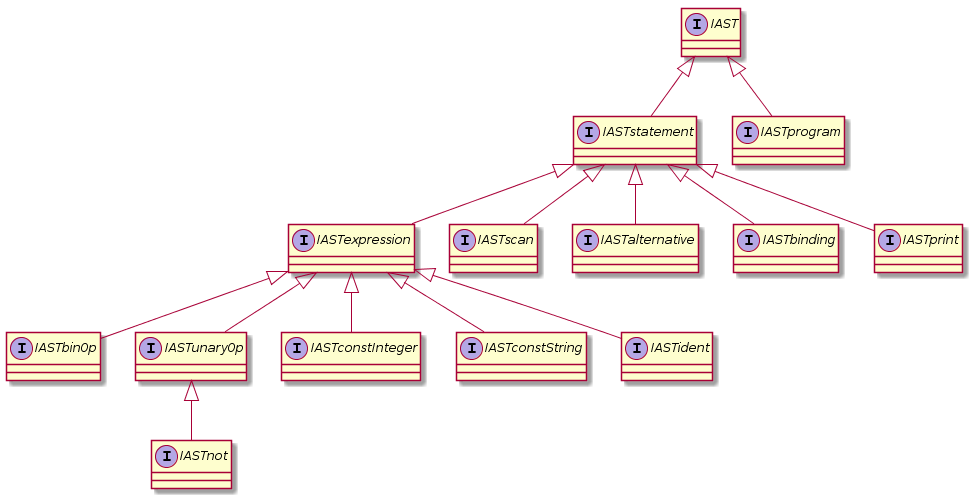
\includegraphics[scale=0.55]{./plantuml/ast_general_structure.png}
 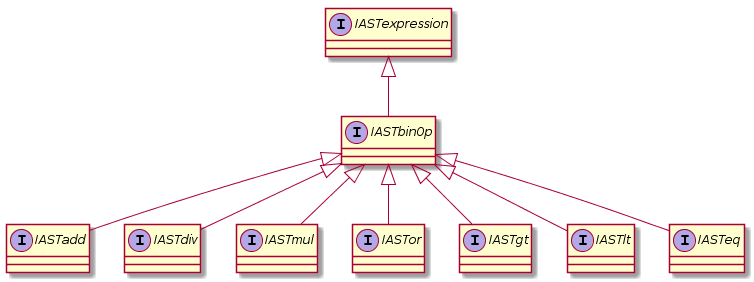
\includegraphics[scale=0.70]{./plantuml/ast_binop_structure.png}
 \begin{figure}
  \caption{Diagramme de classe de la structure générale}
 \end{figure}
\end{center}

Pour générer l'arbre syntaxique abstrait nous avons implantée la classe SUMListener qui réalise l'interface SUMgrammarListener, elle
permet notamment d'appliquer une action à chaque trait du langage reconnut. Nous avons aussi implanté la classe SUMParser qui
initialise et effectue les appels correct afin de construire l'arbre syntaxique abstrait.
Ces classes sont disponibles dans le chemin ./sum/SUM/src/sum/parser.

\section{Compilation vers le langage S-UM}
\subsection{Design Pattern Visitor}
Pour pouvoir parcourir et traité chaque noeud de l'arbre syntaxique abstrait nous avons utilisé le design pattern visitor, ce qui est
très adapté lorsque nous souhaitons faire de l'interpretation/compilation en langage objet. Ainsi, tout les noeuds de l'AST possède
une méthode \textit{public void accept(IASTvisitor visitor)}. L'implantation de la classe Compiler permet lors du parcours de l'AST,
de le compiler.

\subsection{Description générale de la compilation (Class Compiler)}
Les variables suivantes servent à:
\begin{itemize}
 \item NO\_CONTEXT $\rightarrow$ Indiqué lors d'un visit si son évaluation doit être stocké
 \item numInst $\rightarrow$ Permet de savoir le nombre d'instructions écrit (utile pour l'alternative)
 \item env $\rightarrow$ Une Map permettant de garder en mémoire le nom de la variable et l'indice du tableau dans lequel il doit être
 stocké
 \item fos $\rightarrow$ Le flux de sorti
\end{itemize}

\subsection{Stockage des calculs}
Nous avons remarqué qu'il n'y a que 8 registres disponibles, nous sommes donc limités dans le stockage des calculs intermédiaires. Nous
devions, donc trouver un moyen de stockage. Une propriété intéressante est que lors du chargement du programme, seul le tableau[0] est occupé,
ainsi nous savons que les indices libres commencent à partir de 1, de ce fait nous pouvons à l'aide d'une variable entière indVar 
connaitre l'indice de la prochaine allocation puisqu'à chaque allocation on effectue indVar++. Il est important de noter que pour cela 
fonctionne la desallocation ne se fera qu'à la sortie du programme, puisque nous incrémentons à chaque allocation indVar. \\
Cependant, il est possible de désallouer facilement lorsque nous en avons plus besoin, il suffit de garder les indices désalloués dans
une liste, de la même manière que dans la machine universelle. Bien que simple à réaliser, pour des raisons de temps nous ne l'avons pas implanté.
Chaque méthode visit possède un argument \textit{int context}, celui-ci indique si différent de \textit{NO\_CONTEXT} le tableau 
dans lequel le résultat doit être stocké.
La méthode allocateVar() traduit en langage UM, l'instruction d'allocation de taille 1 (puisque l'on stocke unique une valeur).

\subsection{Traduction en instruction UM}
Traduire en directement en binaire UM n'est pas chose aisé, c'est pour cela que nous avons définit des méthodes pour pouvoir traduire
plus facilement.
Les méthodes ci-dessous permettent:
\begin{itemize}
 \item public void writeOperation(int op, int regA, int regB, int regC) $\rightarrow$ Permet d'écrire l'opération op avec les registres
 a,b et c en binaire UM dans le fichier de sorti, on écrit des bytes en utilisant des décalages. (Plus de détail dans le fichier Compiler
 en commentaire).
 \item public void writeSpecialOperation(int regA, int value) $\rightarrow$ Permet de charger une valeur non signé sur 25 bits dans 
 le registre A. (Plus de détail dans le fichier Compiler en commentaire)
 \item public void fetchIntoReg(int i, int reg) $\rightarrow$ Récupère une valeur simple situé dans le plateau[i][0] dans le cas d'une variable
 et l'ajoute dans le registre reg.
 \item public void putIntoArray(int i, int reg) $\rightarrow$ Ajoute dans le plateau[i][0] la valeur dans le registre d'indice reg.
 \item public void allocateVar() $\rightarrow$ Alloue un plateau de taille 1 pour une variable.
\end{itemize}

\subsection{Egalité}
Ecrire les relation binaires n'était pas chose aisée, en effet, nous étions très limités dans les opérations possibles.
Cependant, une remarque importante, soit a un entier NAND(a,a) à pour effet d'inverser les bits. Les 0 deviennent 1 et les 1 deviennent
0. \\
Ainsi nous pouvons donc observer que a + NAND(a,a) = 0b11..11, tout les bits sont positionnés à 1. \\
Donc en additionnant ce résultat à 1, on dépasse 32 bits et donc on retourne a 0b00..00. \\
Donc a + NAND(a,a) + 1 = 0b00..00. \\
On peut donc vérifier l'égalité a = b par: \\
si a + NAND(b,b) + 1 = 0b00..00 alors a = b sinon a != b.
\\ \\
Schéma de compilation: context = (expr1 = expr2);

\begin{verbatim}
  int contextarg1 = indVar++
  allocateVar()
  int contextarg2 = indVar++
  allocateVar()
  tableau[contextarg1][0] <- expr1
  tableau[contextarg2][0] <- expr2
  reg[0] <- tableau[contextarg1][0]
  reg[1] <- tableau[contextarg2][0]
  reg[2] <- NAND(1,1)
  reg[3] <- 1
  reg[2] <- reg[2] + reg[3]
  reg[0] <- reg[0] + reg[2]
  reg[1] <- 1
  reg[2] <- 0
  reg[1] <- if reg[0] = 0 then reg[1] else reg[2]
  tableau[context][0] <- reg[1]
\end{verbatim}

\subsection{Relation d'ordre: > et <}
Pour calculer la relation d'ordre a > b, il suffit simplement de faire une division entière.
Si a/b > 0 alors la relation est vraie, cependant, il y a certaines mesures à prendre,
il faut aussi vérifier le cas où a = b nous réutilisons la code IASTeq. De plus, dans le cas ou le dénominateur b = 0, nous divisons
par 0, pour palier cela le calcul à considérer sera (a+1)/(b+1). Cela ne change pas la relation car si a/b > 0 alors (a+1)/(b+1) aussi.
\\ \\
Schéma de compilation: context = (expr1 / expr2)
\begin{verbatim}
  int contextarg1 = indVar++
  allocateVar()
  int contextarg2 = indVar++
  allocateVar()
  
  tableau[contextarg1][0] <- expr1
  tableau[contextarg2][0] <- expr2
  reg[1] <- tableau[contextarg1][0]
  reg[2] <- tableau[contextarg2][0]
    
  //on ajoute 1 pour eviter la division par 0
  reg[3] <- 1
  reg[1] <- reg[1] + reg[3]
  reg[2] <- reg[2] + reg[3]
    
  //si reg[1]/reg[2] = 0 alors reg[1] < reg[2] car c'est une division entiere
  reg[3] <- reg[1]/reg[2]
  reg[0] <- 0
  reg[4] <- 1
  reg[0] <- if reg[3] != 0 then reg[4] else reg[0]
    
  //on verifie que reg[1] != reg[2]
  //ce sont les mêmes opérations que pour IASTeq
  reg[3] <- NAND(reg[2], reg[2])
  reg[4] <- 1
  reg[3] <- reg[3] + reg[4]
  reg[1] <- reg[3] + reg[1]
  reg[2] <- 1
  reg[3] <- 0
  
  reg[2] <- if reg[1] != 0 then reg[3] else reg[2]
  reg[1] <- 0
  reg[0] <- if reg[2] != 0 then reg[1] else reg[0]
    
  tableau[context][0] <- reg[0]
		
\end{verbatim}
Le code pour l'operation < est identique sauf que l'on change:
\begin{verbatim}
 tableau[contextarg2][0] <- expr1
 tableau[contextarg1][0] <- expr2
\end{verbatim}

\subsection{Or}
La traduction du OR est relativement simple, il suffit de calculer le membre gauche et droit.
A l'aide de l'opération 0 (mouvement conditionnel), nous déterminons si le résultat est 1 (vrai) ou faux (0).
\\ \\
Schéma de compilation: context = (expr1 OR expr2)
\begin{verbatim}
  int contextarg1 = indVar++
  allocateVar()
  int contextarg2 = indVar++
  allocateVar()
  tableau[contextarg1][0] <- expr1
  tableau[contextarg2][0] <- expr2
  reg[1] <- tableau[contextarg1][0]
  reg[2] <- tableau[contextarg2][0]
  reg[0] <- 0
  reg[3] <- 1
  //reg[1] et reg[2] contiennent le resultat de membre gauche et droit de OR
  //reg[0] contient 0, si reg[1] ou reg[2] contiennent la valeur != 0 alors
  //on met dans reg[0] la valeur 1, donc ceci est bien un OR
  reg[0] <- if reg[1] != 0 then reg[3] else reg[0]
  reg[0] <- if reg[1] != 0 then reg[2] else reg[0]
  tableau[context][0] <- reg[0]
\end{verbatim}

\subsection{And}
La traduction du And est très similaire à la traduction du Or, en effet, il y a juste une modification au niveau des mouvements
conditionnels. En effet, nous faisons un ``chainage'' de mouvement conditionnel, ainsi reg[1] et reg[2] (registres qui contiennent le
résultat de l'évaluation des expressions) doivent tout les deux différents de 0 pour que le résultat soit 1 (vrai).
\\ \\
Schéma de compilation: context = (expr1 AND expr2)
\begin{verbatim}
  int contextarg1 = indVar++
  allocateVar()
  int contextarg2 = indVar++
  allocateVar()
  tableau[contextarg1][0] <- expr1
  tableau[contextarg2][0] <- expr2
  reg[2] <- expr1
  reg[3] <- expr2
  reg[4] <- 1
  reg[5] <- 0
  reg[1] <- 0
  reg[0] <- 0
  //reg[2] et reg[3] contiennent le resultat du membre gauche et droit de AND
  //reg[1] = 0 si reg[2] != 0 alors reg[1] = 1
  //reg[0] = 0 si reg[3] != 0 alors reg[0] = reg[1]
  //donc si on a 0 AND 1, reg[0] = 0 etc
  reg[1] <- if reg[2] != 0 then reg[4] else reg[1]
  reg[0] <- if reg[3] != 0 then reg[1] else reg[0]
  tableau[context][0] <- reg[0]
\end{verbatim}

\subsection{Not}
La traduction du Not en UM est très simple, nous utilisons juste un mouvement conditionnel, si la valeur est différent de 0 alors 1 
sinon 0.
\\ \\
Schéma de compilation: context = Not (expr)
\begin{verbatim}
  int argcontext = indVar++
  allocateVar()
  tableau[argcontext][0] <- expr
  reg[2] <- tableau[argcontext][0]
  reg[0] <- 1
  reg[1] <- 0
  //si le resultat est != 0 alors on met 1 sinon 0
  reg[0] <- if reg[2] != 0 then reg[1] else reg[0]
  tableau[context][0] <- reg[0]
\end{verbatim}

\subsection{Operation arithmétique}
Les opérations arithmétiques correspondent juste à un chargement de valeur, l'application de l'opérande et au stockage du résultat.
\\ \\
Schéma de compilation: context = (expr1 [+*/] expr2)
\begin{verbatim}
  int contextarg1 = indVar++;
  allocateVar();
  int contextarg2 = indVar++;
  allocateVar();
  tableau[contextarg1][0] <- expr1
  tableau[contextarg2][0] <- expr2
  reg[0] <- tableau[contextarg1][0]
  reg[1] <- tableau[contextarg2][0]
  reg[2] <- reg[0] [+*/] reg[1]
  tableau[context][0] <- reg[2]
\end{verbatim}


\subsection{Alternative}
L'alternative à une compilation très intéressante à étudier, nous avons essayé dans un premier temps de calculer dynamique le nombre
d'instruction à sauter pour les conditions. Cependant cela n'a pas été concluant, nous avons donc décidé d'alloué les blocs du 
conséquent et de l'alternative à une taille fixe, ce qui rend la détermination des sauts d'adresses relativement plus simple.
Ainsi, l'alternative utilise les opérations de mouvements conditionnels pour déterminer quel saut il faut éffectuer mais aussi des
opérations de chargement de programme permettant de produire des sauts d'instructions.
Nous utilisons ici une variable numInst afin de déterminer les adresses de sauts, numInst est incrémenté à chaque opération écrite.
\\ \\
Schéma de compilation: if expr1 then expr2 else expr3
\begin{verbatim}
  int DEFAULT_SIZE = 4096
  int condctx = indVar++
  allocateVar()
  tableau[condctx][0] <- expr1
  
  //suivant la valeur de la condition, on saute soit a l'adresse du then
  //ou alors a l'adresse du else
  //les blocs de then et else sont fixés, ce qui permet de calculer
  //directement les adresses de sauts
  reg[1] <- numInst+8 //then
  reg[0] <- numInst+8+DEFAULT_SIZE-1 //else
  reg[2] <- tableau[condctx][0]
  
  reg[0] <- if reg[2] != 0 then reg[1] else reg[0]
  reg[1] <- 0
  
  //on charge le programme tableau[reg[1]] et pointe sur la valeur de reg[0]
  //l'instruction qui sera éxécuté au tour prochain sera tableau[reg[1]][reg[0]]
  LOAD_PROG(reg[0], reg[1])
    
  //instructions du then
  int start = numInst;
  NO_CONTEXT <- expr2
    
  //saut hors du if
  reg[1] <- 0
  reg[0] <- start+2*DEFAULT_SIZE
  LOAD_PROG(reg[0],reg[1])
    
  //on remplit le reste du bloc avec des NOP
  while(numInst < start+DEFAULT_SIZE) {
    reg[0] <- 0
  }
    
  //instructions du else
  NO_CONTEXT <- expr3
    
  //on remplit le reste du bloc avec des NOP
  while(numInst < start+2*DEFAULT_SIZE) {
    reg[0] <- 0
  }
\end{verbatim}


\subsection{Binding}
Le binding est une déclaration de variable, ainsi nous l'ajoutons dans l'environnement de compilation dans une map le nom et l'indice
du tableau dont on l'a attribué, s'il est déclaré avec une expression le calcul de l'expression y sera stocké.
\\ \\
Schéma de compilation: let var = expr
\begin{verbatim}
  int varcontext = indVar++
  allocateVar()
  env.put(var, varcontext)
  if existExpr() then tableau[varcontext][0] <- expr
\end{verbatim}

\subsection{Ident}
Les ident correspondent aux noms de variable, nous gardons dans l'environnement de compilation une map contenant le nom de la variable
et l'indice du tableau dans laquelle est stocké la variable.
\\ \\
Schéma de compilation: context = expr
\begin{verbatim}
  int varcontext = env.get(expr)
  reg[0] <- tableau[varcontext][0]
  tableau[context] <- reg[0]
\end{verbatim}


\subsection{Integer}
La traduction de la constante est trivial, cela correspond au chargement de la valeur immédiate dans une case du tableau.
\\ \\
Schéma de compilation: context = expr
\begin{verbatim}
  reg[0] <- expr
  tableau[context][0] <- reg[0]
\end{verbatim}

\section{Tests}
Le jeux de tests se trouve dans le dossier ./tests, ce sont des tests unitaires de chaque trait du langage.
Nous effectuons principalement des tests avec des affichages attendus, étant donné que l'affiche d'une expression est sous forme ASCII,
nous verifions dans la plupart des cas que la valeur correspond bien à une lettre attendue.
Cependant d'autres tests, plus élaborés sont disponibles mais ne sont pas au format demandé, ces tests se trouve dans les sources 
du compilateur S-UM, dans le chemin ./sum/SUM/test.

\end{document}

